\documentclass{beamer}
\setbeamersize{text margin left=3mm,text margin right=3mm}

\usepackage[backend=bibtex, natbib=true, style=authoryear]{biblatex}% \usepackage[style=authoryear]{natbib}
% \bibliographystyle{plain}
\addbibresource{bibliography}

\usepackage{amsmath, bm, amssymb}
\usepackage{tcolorbox}
\usepackage{graphicx}
\usepackage{xcolor}
\usepackage{listings}
%New colors defined below
\definecolor{codegreen}{rgb}{0,0.6,0}
\definecolor{codegray}{rgb}{0.5,0.5,0.5}
\definecolor{codepurple}{rgb}{0.58,0,0.82}
\definecolor{backcolour}{rgb}{0.95,0.95,0.92}

%Code listing style named "mystyle"
\lstdefinestyle{mystyle}{
  backgroundcolor=\color{backcolour}, commentstyle=\color{codegreen},
  keywordstyle=\color{magenta},
  numberstyle=\tiny\color{codegray},
  stringstyle=\color{codepurple},
  basicstyle=\ttfamily\footnotesize,
  breakatwhitespace=false,
  breaklines=true,
  captionpos=b,
  keepspaces=true,
  numbers=left,
  numbersep=5pt,
  showspaces=false,
  showstringspaces=false,
  showtabs=false,
  tabsize=2
}
\lstset{style=mystyle}


\usepackage{hyperref}
\hypersetup{
    colorlinks=true,
    linkcolor=blue,
    filecolor=magenta,
    urlcolor=cyan,
    pdftitle={Overleaf Example},
    pdfpagemode=FullScreen,
    }
\usepackage{multirow}
\usetheme{Boadilla}
\usecolortheme{seahorse}
\newcommand{\thetab}{\boldsymbol{\theta}}
\newcommand{\xb}{\boldsymbol{x}}
\newcommand{\red}[1]{\textcolor{red}{#1}}
\newcommand{\blue}[1]{\textcolor{blue}{#1}}

\DeclareMathOperator*{\argmin}{arg\,min}
\DeclareMathOperator*{\argmax}{arg\,max}

\title[TaDA workshop - VLDB 2024]{TaDA workshop - VLDB 2024}
\subtitle{Fast and accurate regional effect plots for automated tabular
data analysis}
\author[Gkolemis, Vasilis] % (optional)
{Vasilis Gkolemis\inst{1,2} \and
  Christos Diou\inst{2} \and
  Eirini Ntoutsi\inst{3} \and
  Theodore Dalamagas\inst{1}
}

\institute[ATH-HUA]{
  \inst{1} ATHENA Research and Innovation Center
  \and %
  \inst{2} Harokopio University of Athens
  \and
  \inst{3} University of the Bundeswehr Munich
}

\date{August 2024}


% Use a simple TikZ graphic to show where the logo is positioned
% \logo{\begin{tikzpicture}
% \filldraw[color=red!50, fill=red!25, very thick](0,0) circle (0.5);
% \node[draw,color=white] at (0,0) {LOGO HERE};
% \end{tikzpicture}}

%End of title page configuration block
%------------------------------------------------------------
%The next block of commands puts the table of contents at the
%beginning of each section and highlights the current section:

\AtBeginSection[]
{
  \begin{frame}
    \frametitle{Program}
    \tableofcontents[currentsection]
  \end{frame}
}
\AtBeginSubsection[]
{
  \begin{frame}
    \frametitle{Program}
    \tableofcontents[currentsubsection]
  \end{frame}
}


% ------------------------------------------------------------
\begin{document}
\frame{\titlepage}
%---------------------------------------------------------


\section{Introduction}

\subsection{Problem Statement}

\begin{frame}
  \frametitle{Problem Statement}
  \begin{figure}[ht]
    \centering
    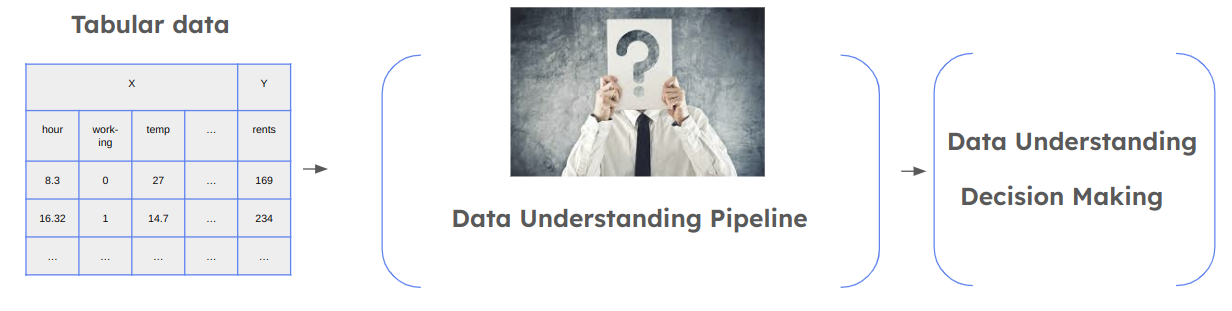
\includegraphics[width=\textwidth]{./figures/problem_statement.png}
  \end{figure}
  \noindent\makebox[\linewidth]{\rule{\paperwidth}{0.4pt}}
  I will try to convince you for 4 things!
\end{frame}

\subsection{Proposed Pipeline}

\begin{frame}
  \frametitle{Discussion point 1}
  \begin{figure}[ht]
    \centering
    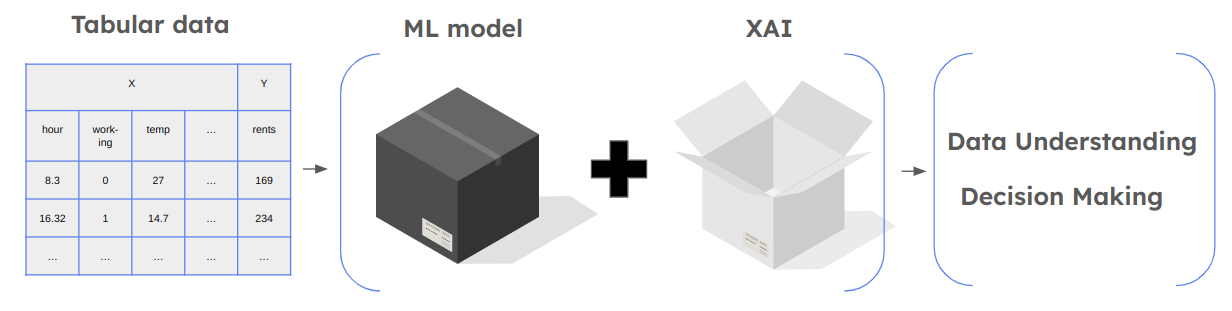
\includegraphics[width=\textwidth]{./figures/convincing_point_1.png}
  \end{figure}
  \noindent\makebox[\linewidth]{\rule{\paperwidth}{0.4pt}}
  Black box ML model + XAI = a good pipeline!
\end{frame}

\begin{frame}
  \frametitle{Discussion point 2}
  \begin{figure}[ht]
    \centering
    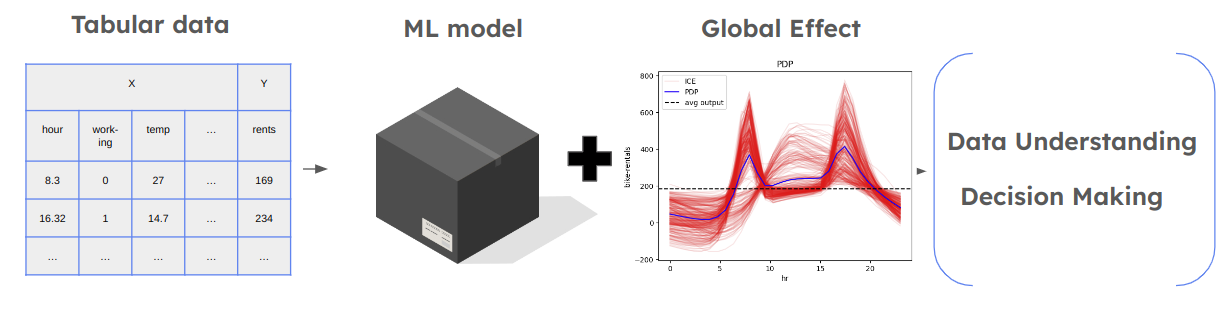
\includegraphics[width=\textwidth]{./figures/convincing_point_2.png}
  \end{figure}
  \noindent\makebox[\linewidth]{\rule{\paperwidth}{0.4pt}}
  Black box ML model + Global effect methods = a good pipeline!
\end{frame}

\begin{frame}
  \frametitle{Discussion point 3}
  \begin{figure}[ht]
    \centering
    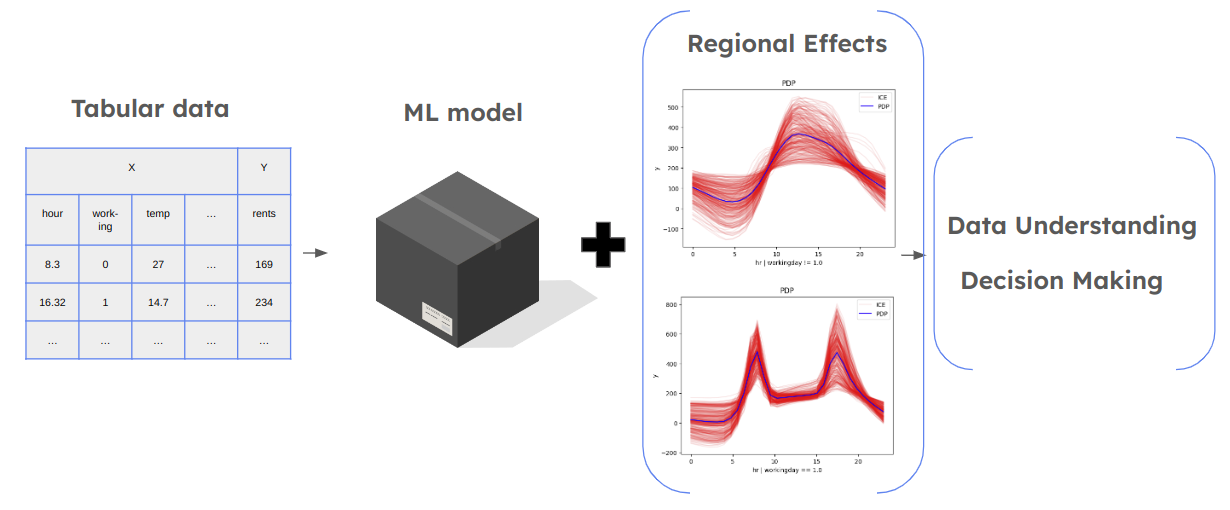
\includegraphics[width=\textwidth]{./figures/convincing_point_3.png}
  \end{figure}
  \noindent\makebox[\linewidth]{\rule{\paperwidth}{0.4pt}}
  Black box ML model + Regional effect methods = a better pipeline!
\end{frame}

\begin{frame}
  \frametitle{Discussion point 4}
  \begin{figure}[ht]
    \centering
    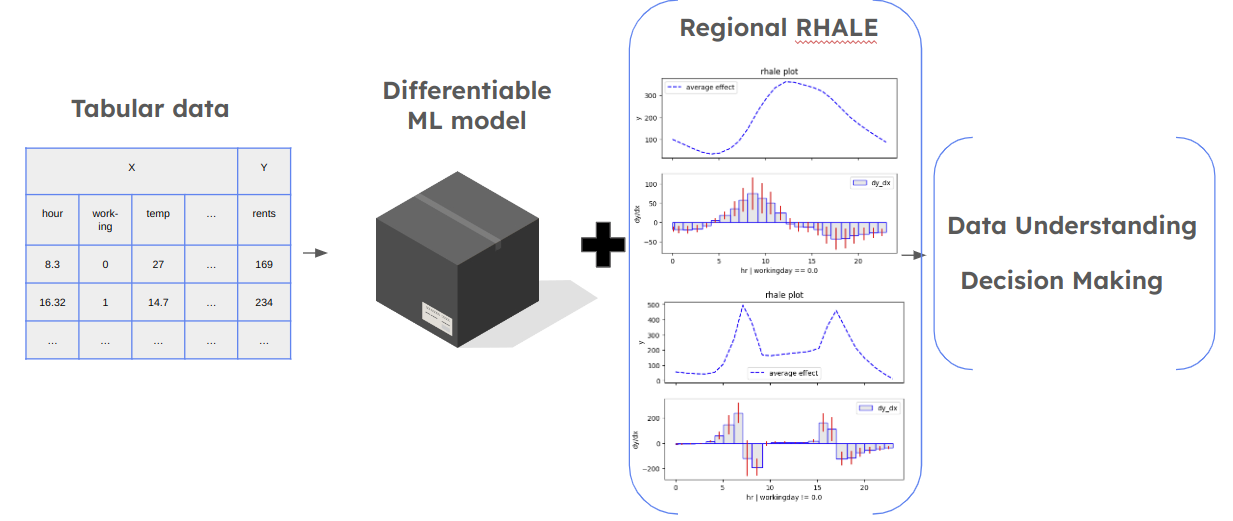
\includegraphics[width=\textwidth]{./figures/convincing_point_4.png}
  \end{figure}
  \noindent\makebox[\linewidth]{\rule{\paperwidth}{0.4pt}}
  Black box ML model + Regional RHALE = an even better pipeline!
\end{frame}

% \begin{frame}
%   \frametitle{Feature Effect}
%   \begin{itemize}
%     \item $f(\cdot): \mathbf{x} \rightarrow y \longrightarrow f_i(\cdot): x_i \rightarrow y \: \forall i $
%   \end{itemize}
%   \vspace{2mm}
%   \begin{figure}[ht]
%     \centering
%     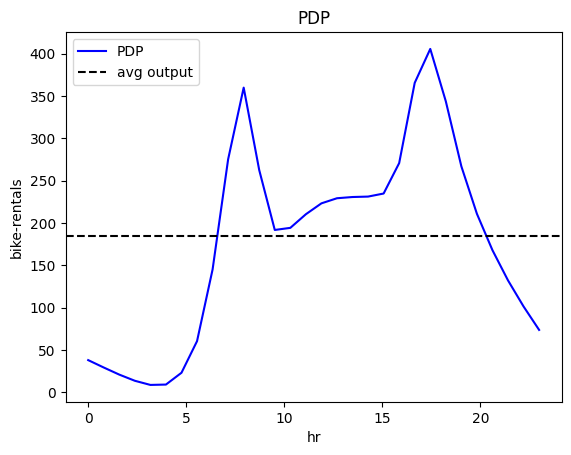
\includegraphics[width=0.5\textwidth]{./figures/bike_sharing_global_pdp.png}
%   \end{figure}

%   \noindent\makebox[\linewidth]{\rule{\paperwidth}{0.4pt}}
%   Simple and intuitive.
% \end{frame}

% \section{Feature Effect}
% \subsection{Bike-sharing dataset}

\begin{frame}
  \frametitle{Bike-sharing dataset}
  \begin{itemize}
  \item hourly count of bike-rentals (2011, 2012)
  \item Design-matrix $X$:
    \begin{itemize}
    \item year, month, day, \red{hour}
    \item working day vs. non-working day
    \item temperature
    \item humidity
    \item windspeed
    \end{itemize}
  \item Target variable $Y$:
    \begin{itemize}
    \item bike-rentals per hour
      \begin{itemize}
      \item $Y_\mu = 189.5$
      \item $Y_\sigma = 181.4$
      \end{itemize}
    \end{itemize}
  \item Decision Making: \red{decide a discount policy}
  \item Data Understanding: confirm/reject some ideas about bike rentals
  \end{itemize}
\end{frame}


\begin{frame}
  \frametitle{Proposed pipeline: Fit and Explain}
  \begin{itemize}
  \item \red{decide a discount policy}
    \begin{itemize}
    \item which hour of the day to apply the discount
    \item how the feature $x_{\mathtt{hour}}$ relates to $y_{\mathtt{bike\_rentals}}$
    \end{itemize}

  \item Step 1: Fit a black-box ML model
    \begin{itemize}
    \item Could be any ML model
    \item a Neural Network achieves $\texttt{RMSE} \approx 45.35 $ counts ($0.25Y_\sigma$)
    \end{itemize}
  \item Step 2: Use feature effect
    \begin{itemize}
    \item Global effect: $x_{\mathtt{hour}}$ vs $y_{\mathtt{bike\_rentals}}$ globally
    \item Regional effect: $x_{\mathtt{hour}}$ vs $y_{\mathtt{bike\_rentals}}$ regionally
    \end{itemize}
  \end{itemize}

  \noindent\makebox[\linewidth]{\rule{\paperwidth}{0.4pt}}
  Let's see!
\end{frame}

\begin{frame}
  \frametitle{Global Effect: PDP and RHALE}
  \begin{figure}[ht]
    \centering
    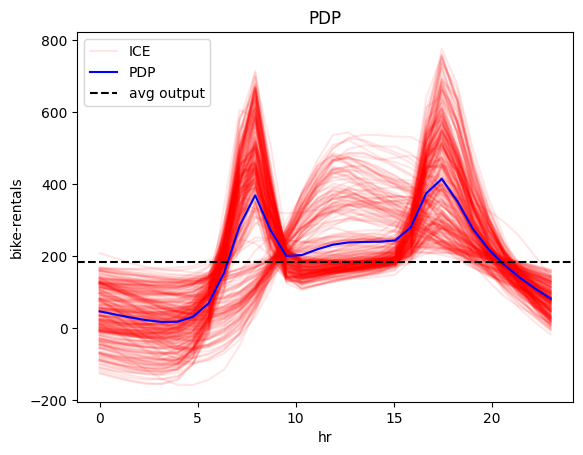
\includegraphics[width=0.45\textwidth]{./figures/bike_sharing_global_pdp_heterogeneity.png}
    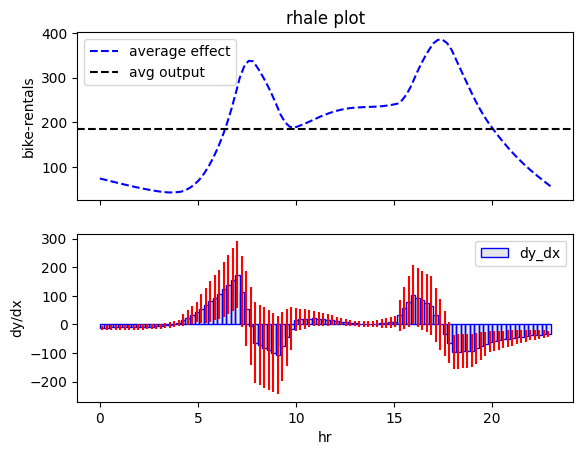
\includegraphics[width=0.45\textwidth]{./figures/bike_sharing_global_rhale_heterogeneity.png}
  \end{figure}
  \noindent\makebox[\linewidth]{\rule{\paperwidth}{0.4pt}}
  RHALE paper~\citep{gkolemis2023rhale}: ALE + heterogeneity
\end{frame}

\begin{frame}
  \frametitle{Regional Effect: Regional-PDP}
  \begin{figure}[ht]
    \centering
    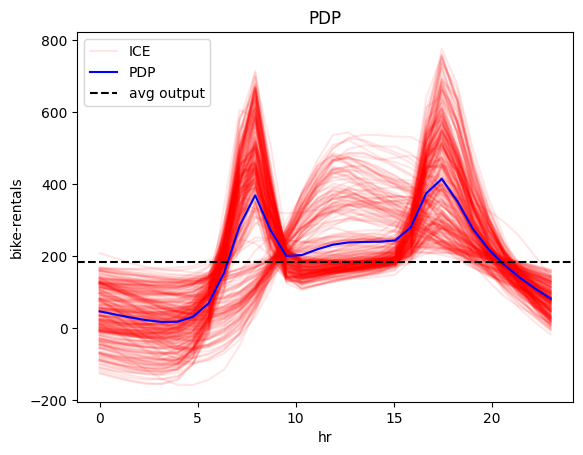
\includegraphics[width=0.33\textwidth]{./figures/bike_sharing_global_pdp_heterogeneity.png}\\
    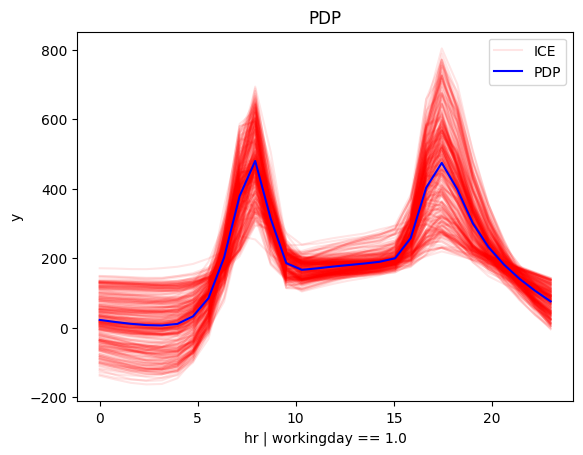
\includegraphics[width=0.33\textwidth]{./figures/bike_sharing_regional_pdp_workingdays.png}
    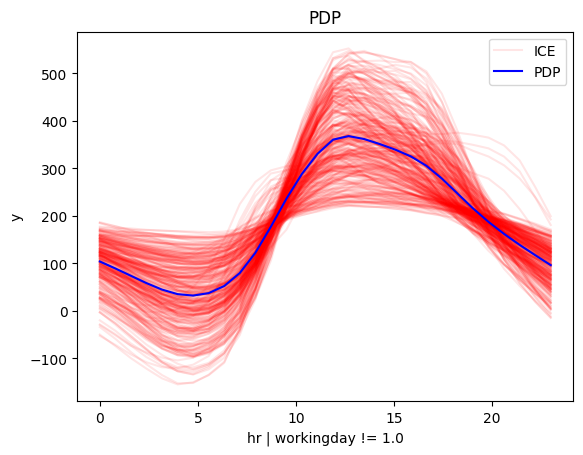
\includegraphics[width=0.33\textwidth]{./figures/bike_sharing_regional_pdp_weekends.png}
  \end{figure}
  \noindent\makebox[\linewidth]{\rule{\paperwidth}{0.4pt}}
  REPID Paper~\citep{herbinger_repid_2022}
\end{frame}

\subsection{Regional RHALE - our contribution}
\begin{frame}
  \frametitle{Regional Effect: Regional-RHALE}
  \begin{figure}[ht]
    \centering
    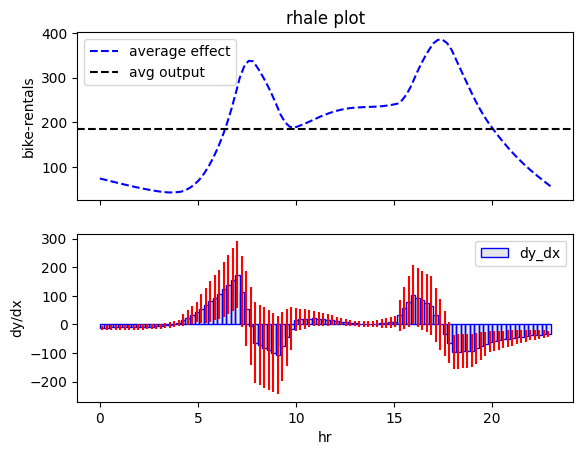
\includegraphics[width=0.33\textwidth]{./figures/bike_sharing_global_rhale_heterogeneity.png} \\
    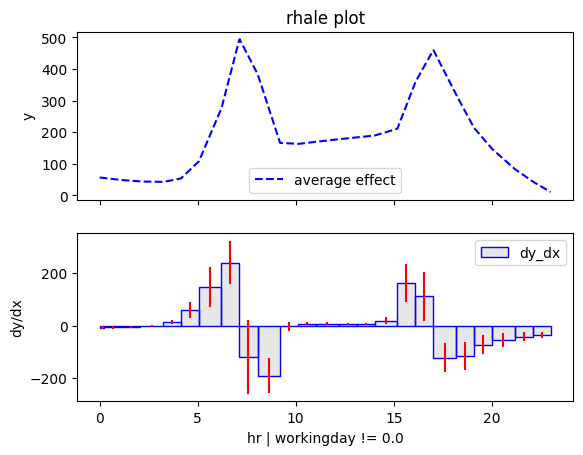
\includegraphics[width=0.33\textwidth]{./figures/bike_sharing_regional_rhale_workingdays.png}
    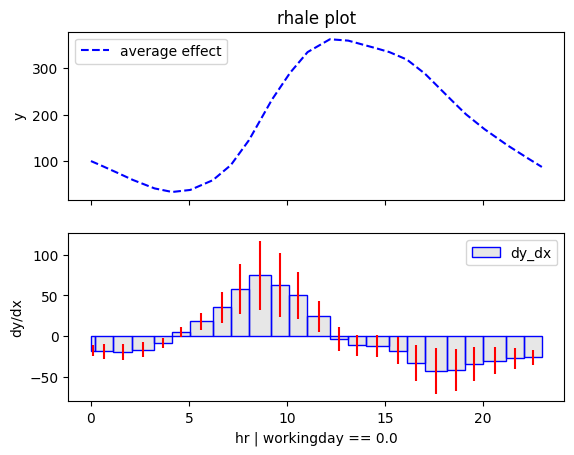
\includegraphics[width=0.33\textwidth]{./figures/bike_sharing_regional_rhale_weekends.png}
  \end{figure}
  \noindent\makebox[\linewidth]{\rule{\paperwidth}{0.4pt}}
  Regional RHALE - our proposal!
\end{frame}

\section{Regional RHALE - advantages}

\subsection{It is fast}

\subsection{It treats well correlated features}

\section{Effector - Python package}

% \section{\texttt{Effector}}

% \begin{frame}
%   \frametitle{Why \texttt{Effector}?}
%   \begin{itemize}
%   \item Regional Methods
%   \item Fast
%   \item Integrates with all frameworks
%   \item Common API between methods
%   \item Progressive disclosure of complexity
%   \item Extensible
%   \end{itemize}
% \end{frame}

% \subsection{Regional Methods}
% \begin{frame}
%   \frametitle{Regional Methods}
%   \begin{itemize}
%   \item only package with regional effect methods
%   \end{itemize}
%   \begin{figure}
%     \centering
%     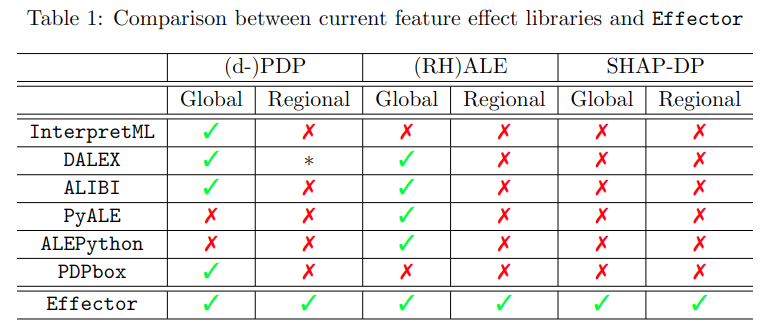
\includegraphics[width=0.8\textwidth]{./figures/effector_comparison.png}
%   \end{figure}
%   \begin{itemize}
%   \item will keep being updated with novel methods!
%   \end{itemize}
% \end{frame}

% \subsection{Fast}
% \begin{frame}
%   \frametitle{Fast}
%   \begin{figure}[ht]
%     \centering
%     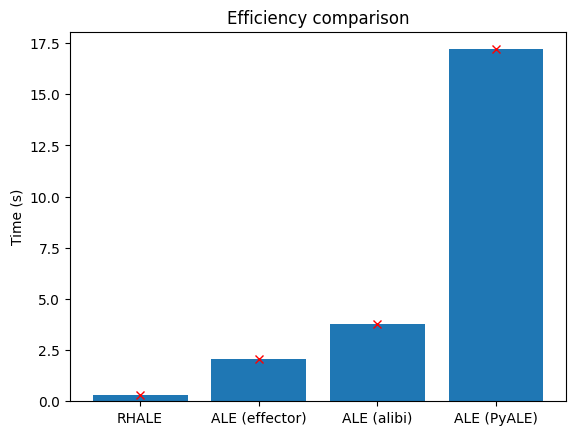
\includegraphics[width=0.5\textwidth]{./figures/efficiency_comparison.png}
%     \caption{ALE-based plots on bike-sharing dataset}
%     \end{figure}
%   \noindent\makebox[\linewidth]{\rule{\paperwidth}{0.4pt}}
%   \begin{itemize}
%   \item RHALE is a very fast method
%   \item \texttt{Effector} focuses on efficiency $\rightarrow$ regional methods
%   \end{itemize}
% \end{frame}

% \subsection{Integrates with all frameworks}
% \begin{frame}[fragile]
% \frametitle{\texttt{Effector} is simple: Scikit-learn}

% \begin{lstlisting}[language=Python]
% import effector
% from sklearn.ensemble import RandomForestRegressor

% # X = ... # input data
% # y = ... # target data

% model = RandomForestRegressor()
% model.fit(X, y)

% def f(X):
%   return model.predict(X)

% # global effect
% effector.PDP(X, f).plot(feature=0)

% # regional effect
% effector.RegionalPDP(X, f).plot(feature=0, node_idx=0)
% \end{lstlisting}
% \end{frame}

% \begin{frame}[fragile]
% \frametitle{\texttt{Effector} is simple: Tensorflow - (i)}

% \begin{lstlisting}[language=Python]
% import effector
% import tensorflow as tf

% # X = ... # input data
% # y = ... # target data

% # define model
% model = tf.keras.Sequential([
%   tf.keras.layers.Dense(10, activation='relu'),
%   tf.keras.layers.Dense(1)
% ])

% # train model
% model.compile(optimizer='adam', loss='mse')
% model.fit(X, y, epochs=10)
% \end{lstlisting}
% \end{frame}

% \begin{frame}[fragile]
% \frametitle{\texttt{Effector} is simple: Tensorflow - (ii)}

% \begin{lstlisting}[language=Python]
% def f(X):
%   return model.predict(X)

% def f_jac(X):
%     X = tf.convert_to_tensor(X, dtype=tf.float32)
%     with tf.GradientTape() as tape:
%         tape.watch(X)
%         y = model(X)
%     return tape.gradient(y, X).numpy()

% # global effect
% effector.RHALE(X, f, f_jac).plot(feature=0)

% # regional effect
% effector.RegionalRHALE(X, f, f_jac).plot(feature=0, node_idx=0)
% \end{lstlisting}
% \end{frame}

% \begin{frame}[fragile]
% \frametitle{\texttt{Effector} is simple: PyTorch - (i)}

% \begin{lstlisting}[language=Python]
% import effector
% import torch
% import torch.nn as nn

% # X = ... # input data
% # y = ... # target data

% class Net(nn.Module):
%   def __init__(self):
%     super(Net, self).__init__()
%     self.fc1 = nn.Linear(D, 10)
%     self.fc2 = nn.Linear(10, 1)

%   def forward(self, x):
%     x = self.fc1(x)
%     x = self.fc2(x)
%     return x

% model = Net()
% \end{lstlisting}
% \end{frame}

% \begin{frame}[fragile]
% \frametitle{\texttt{Effector} is simple: PyTorch - (ii)}

% \begin{lstlisting}[language=Python]
% # train model
% optimizer = torch.optim.Adam(model.parameters(), lr=0.01)
% criterion = nn.MSELoss()
% for epoch in range(10):
%   optimizer.zero_grad()
%   y_pred = model(X)
%   loss = criterion(y_pred, y)
%   loss.backward()
%   optimizer.step()
% \end{lstlisting}
% \end{frame}

% \begin{frame}[fragile]
% \frametitle{\texttt{Effector} is simple: PyTorch - (iii)}

% \begin{lstlisting}[language=Python]
% def f(X):
%     return model(torch.tensor(X, dtype=torch.float32)).detach().numpy()

% def f_jac(X):
%     X = torch.tensor(X, dtype=torch.float32)
%     X.requires_grad = True
%     y = model(X)
%     return torch.autograd.grad(y, X)[0].numpy()

% # global effect
% effector.RHALE(X, f, f_jac).plot(feature=0)

% # regional effect
% effector.RegionalRHALE(X, f, f_jac).plot(feature=0, node_idx=0)
% \end{lstlisting}
% \end{frame}

% \subsection{Common API between methods}
% \begin{frame}[fragile]
% \frametitle{Common API between methods}
% \begin{lstlisting}[language=Python]
% # global effect
% effector.PDP(X, f).plot(feature=i)
% effector.RHALE(X, f, f_jac).plot(feature=i)
% effector.SHAPDP(X, f).plot(feature=i)


% # regional effect
% effector.RegionalPDP(X, f).plot(feature=i, node_idx=0)
% effector.RegionalRHALE(X, f, f_jac).plot(feature=i, node_idx=0)
% effector.RegionalSHAPDP(X, f).plot(feature=i, node_idx=0)
% \end{lstlisting}
% \end{frame}

% \subsection{Progressive disclosure of complexity}
% \begin{frame}
% \frametitle{Progressive disclosure of complexity}
% \begin{figure}
%   \centering
%     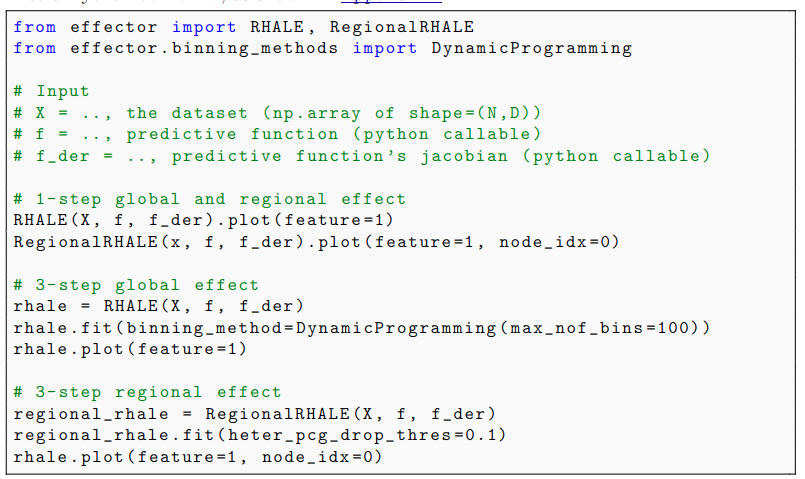
\includegraphics[width=0.9\textwidth]{./figures/effector_disclosure_complexity.png}
% \end{figure}
% \end{frame}


% \subsection{Extensible}
% \begin{frame}
%   \frametitle{Extensibility}
%   \begin{itemize}
%   \item Effector is designed to maximize extensibility
%   \item library is structured around a set of abstractions
%   \item one can easily create a novel ALE-based method
%     \begin{itemize}
%     \item subclass \texttt{ALEBase} class
%     \item redefine the \texttt{.fit()} and/or \texttt{.plot()}
%     \end{itemize}
%   \end{itemize}
% \end{frame}

% \section{Future Directions}

% \begin{frame}
%   \frametitle{Future directions}
%   \begin{itemize}
%   \item On the road to \texttt{v.1}
%     \begin{itemize}
%     \item test, robustify, get feedback
%     \item complete documentation
%     \item add more real-world examples
%     \end{itemize}
%   \item Novel Features
%   \begin{itemize}
%   \item Faster implementation of SHAP-DP
%     \begin{itemize}
%     \item current regional version is prohibitively slow
%     \end{itemize}
%   \item Integration of Regionally Additive Models~\citep{gkolemis2023regionally}
%     \begin{itemize}
%     \item Use subregions to fit an x-by-design model
%     \item RAM $=$ GAM on subregions
%     \end{itemize}
%   \item Benchmark datasets
%     \begin{itemize}
%     \item There is not a single ground truth!
%     \item Design datasets with desiderata
%     \item compare methods
%     \end{itemize}
%   \end{itemize}
% \item Get feedback from the community
% \end{itemize}
% \end{frame}

\begin{frame}
  \frametitle{Thank You!}
  \begin{itemize}
  \item If you find this package useful, we would appreciate your feedback and a star on GitHub
  \item \href{https://arxiv.org/abs/2404.02629}{https://arxiv.org/abs/2404.02629}
  \item \href{https://github.com/givasile/effector}{https://github.com/givasile/effector}
  \item \href{https://xai-effector.github.io/}{https://xai-effector.github.io/}
  \end{itemize}

\end{frame}



\begin{frame}[allowframebreaks]
  \frametitle{References}
  \printbibliography
\end{frame}

\end{document}
